\documentclass[handout]{beamer}


\usetheme{default}
\usepackage{subfigure}
\usepackage{amsmath}
\usepackage{Sweave}
\usepackage{graphicx}
\usepackage{color}
\usepackage{amsfonts}
\usepackage{amssymb}
\usepackage{multicol}
\usepackage[all]{xy}
\usepackage{bm}


\author{Patrick Lam}
\title{Delta Method and Generalized Linear Models}
\date{}
%\date{March 12, 2009}

\begin{document}

\newcommand{\red}{\textcolor{red}}
\newcommand{\blue}{\textcolor{blue}}
\newcommand{\purple}{\textcolor{purple}}
\newcommand{\brown}{\textcolor{brown}}

\frame{\titlepage}

\section{The Delta Method}

\begin{frame}
%\frametitle{The Delta Method}
\pause
Suppose we have a random variable $X$, and we know $E(X)$ and Var($X$).\\
\pause
\bigskip
Let $Y$ be another random variable such that $Y = g(X)$. \\
\pause
\bigskip
How do we find $E(Y)$ and Var($Y$)? \pause (useful for
reparameterizations and quantities of interest) \\
\pause
\begin{itemize}
\item Find $E(Y)$ via $\int_{-\infty}^{\infty} g(x) p(x) dx$
\pause
\item Simulation
\pause
\item Delta Method
\end{itemize}
\end{frame}

\begin{frame}
\frametitle{If g(X) is linear...}
\pause
this is pretty straightforward:
\pause
\begin{eqnarray*}
Y &=& a + bX \\
\pause
E(Y) &=& a + b E(X) \\
\pause
\mathrm{Var}(Y) &=& b^2 \mathrm{Var}(X)
\end{eqnarray*}
\pause
What if g(X) isn't linear? \\
\bigskip
\pause
We will use the \textbf{delta method}, which relies on a linear approximation to $g(X)$ near the mean of $X$.
\end{frame}

\begin{frame}
\frametitle{Delta Method}
\pause
Denote $\mu_X$ as the mean of $X$. \pause We use a first-order
Taylor series approximation around $\mu_X$:
\pause
\begin{eqnarray*}
Y &=& g(X) \\
\pause
&\approx& g(\mu_X) + (X - \mu_X) g'(\mu_X) \\ \\
\pause 
E(Y) &\approx& E[g(\mu_X)] + \red{E[(X - \mu_X) g'(\mu_X)]} \\
\pause
&=& g(\mu_X) \; \mathrm{since \;}E(X-\mu_X) = 0 \\ \\
\pause
\mathrm{Var}(Y) &\approx& \red{\mathrm{Var}[g(\mu_X)]} + \mathrm{Var}[(X -
\mu_X) g'(\mu_X)] \\
\pause
&=& \red{0} + \mathrm{Var}[X g'(\mu_X)] - \red{\mathrm{Var}[\mu_X g'(\mu_X) ]} \\
\pause
&=& \mathrm{Var}(X) [g'(\mu_X)]^2
\end{eqnarray*}

\end{frame}

\begin{frame}
\frametitle{One More Step...}
\pause
We have 
\begin{eqnarray*}
E(Y) &\approx& g(\mu_X)
\end{eqnarray*}
\pause
but we know generally (from Jensen's inequality)
\begin{eqnarray*}
E(g(X)) \neq g(E(X))
\end{eqnarray*} 
\pause
so we use the second order Taylor expansion for $E(Y)$
\pause
\begin{eqnarray*}
Y &\approx& g(\mu_X) + (X - \mu_X) g'(\mu_X) + \frac{1}{2} (X-\mu_X)^2
g''(\mu_X) \\ 
\pause
E(Y) &\approx& E[g(\mu_X)] + \red{E[(X - \mu_X) g'(\mu_X)]} + \frac{1}{2}
E[(X-\mu_X)^2 g''(\mu_X)] \\
\pause
&=& g(\mu_X) + \frac{1}{2} \mathrm{Var}(X) g''(\mu_X)
\end{eqnarray*}
\end{frame}

\begin{frame}
So we have
\begin{eqnarray*}
E(Y) &\approx& g(\mu_X) + \frac{1}{2} \mathrm{Var}(X) g''(\mu_X) \\
\mathrm{Var}(Y) &\approx& \mathrm{Var}(X) [g'(\mu_X)]^2
\end{eqnarray*}
\pause
How good the approximations are depend on how nonlinear $g(X)$ is in
the neighborhood of $\mu_X$ and on the size of Var($X$).
\end{frame}

\section{Generalized Linear Models}

\begin{frame}
\frametitle{Generalized Linear Models}
\pause
All of the models we've talked about so far (and for the rest of the
class) belong to a class called \textbf{generalized linear models (GLM)}.\\
\pause
\bigskip
Three elements of a GLM:
\pause
\begin{itemize}
\item A distribution for $Y$
\pause
\item A linear predictor $X\beta$
\pause
\item A link function that relates the linear predictor to the mean of
the distribution.
\end{itemize}
\pause
\bigskip
Steps to running a GLM:
\end{frame}

\begin{frame}
\frametitle{1. Specify a distribution for $Y$}
\pause
Assume our data was generated from some distribution.\\
\pause
\bigskip
Examples:
\pause
\begin{itemize}
\item Continuous and Unbounded: \pause Normal
\pause
\item Binary: \pause Bernoulli 
\pause
\item Event Count: \pause Poisson
\pause
\item Duration: \pause Exponential
\pause
\item Ordered Categories: \pause Normal with observation mechanism
\pause
\item Unordered Categories: \pause Multinomial
\end{itemize}
\end{frame}

\begin{frame}
\frametitle{2. Specify a linear predictor}
\pause
\begin{eqnarray*}
X \beta = \beta_0 + x_1 \beta_1 + x_2 \beta_2 + \dots + x_k \beta_k
\end{eqnarray*}
\end{frame}

\begin{frame}
\frametitle{3. Specify a link function}
\pause
The link function relates the linear predictor to the mean of the
distribution for $Y$. \\
\bigskip
\pause
Let $g(\cdot)$ be the link function and let $E(Y) = \theta$ be the
mean of distribution for $Y$.  
\pause
\begin{eqnarray*}
g(\theta) &=& X\beta \\
\pause
\theta &=& g^{-1} (X \beta)
\end{eqnarray*}
\pause
Note that we usually use the \textbf{inverse link function} $g^{-1}(X
\beta)$ rather than the link function. \\
\pause
\bigskip
This is the systematic component that we've been talking about all along.
\end{frame}

\begin{frame}
\frametitle{Example Link Functions}
\pause
\footnotesize
Identity: 
\pause
\begin{itemize}
\item Link: $\mu = X\beta$ 
\pause
 \item Inverse Link: $\mu = X\beta$
\end{itemize}
\pause
Inverse:
\pause
\begin{itemize}
\item Link: $\lambda^{-1} = X\beta$
\pause 
\item Inverse Link:  $\lambda = (X\beta)^{-1}$
\end{itemize}
\pause
Logit: 
\pause
\begin{itemize}
\item Link: $\mathrm{ln} \left( \frac{\pi}{1-\pi} \right) = X\beta$
\pause 
\item Inverse Link: $\pi = \frac{1}{1 + e^{-X\beta}} $
\end{itemize}
\pause
Probit: 
\pause
\begin{itemize}
\item Link: $\Phi^{-1}(\pi) = X\beta$
\pause 
\item Inverse Link: $\pi = \Phi(X\beta) $
\end{itemize}
\pause
Log:
\pause
\begin{itemize}
\item Link: $\mathrm{ln}(\lambda) = X\beta$
\pause 
\item Inverse Link: $\lambda = \exp(X\beta) $
\end{itemize}
\end{frame}

\begin{frame}
\frametitle{4. Estimate Parameters via ML}
\pause
Do it.
\end{frame}

\begin{frame}
\frametitle{5. Quantities of Interest}
\pause
\begin{enumerate}
\item Simulate parameters from multivariate normal.
\pause
\item Run $X\beta$ through inverse link function to get expected values.
\pause
\item Draw from distribution of $Y$ for predicted values.
\end{enumerate}
\end{frame}

\subsection{Binary Dependent Variable Models}

\begin{frame}
\frametitle{Binary Dependent Variable}
Let our dependent variable be a binary random variable that can take
on values of either 0 or 1.
\end{frame}

\begin{frame}
\begin{enumerate}
\item Specify a distribution for $Y$
\end{enumerate}
\pause
\begin{eqnarray*}
Y_i &\sim& \mathrm{Bernoulli}(\pi_i) \\
\pause
p(\mathrm{y} | \bm{\pi}) &=& \prod^n_{i=1} \pi_i^{y_i} (1-\pi_i)^{1-y_i}
\end{eqnarray*}
\pause
\begin{itemize}
\item[2.] Specify a linear predictor: \pause $X\beta$
\end{itemize}
\end{frame}

\begin{frame}
\begin{itemize}
\item[3.] Specify a link (or inverse link) function.
\pause
\begin{itemize}
\item Logit: $\pi_i = \frac{1}{1+e^{-x_i\beta}}$
\pause
\item Probit: $\pi_i = \Phi(x_i \beta)$
\pause
\item Complementary Log-log (cloglog): $\pi_i = 1 - \exp(-\exp(X\beta))$
\pause
\item Scobit: $\pi_i = (1+e^{-x_i \beta})^{-\alpha}$
\end{itemize}
\pause
\bigskip
\item[4.] Estimate parameters via ML.
\pause
\end{itemize}
\begin{eqnarray*}
l(\beta | \mathbf{y}) &=& \sum^n_{i=1} y_i \; \mathrm{ln} \,
\left(\frac{1}{1+e^{-x_i\beta}}\right) + (1-y_i) \; \mathrm{ln} \, \left(1-\frac{1}{1+e^{-x_i\beta}}\right)
\end{eqnarray*}
\pause
\begin{itemize}
\item[5.] Simulate Quantities of Interest
\end{itemize}
\end{frame}

\subsection{Ordinal Dependent Variable Models}

\begin{frame}
\frametitle{Identification}
\pause
Suppose we have the following log-likelihood function:
\begin{figure}[!htp]
\begin{center}
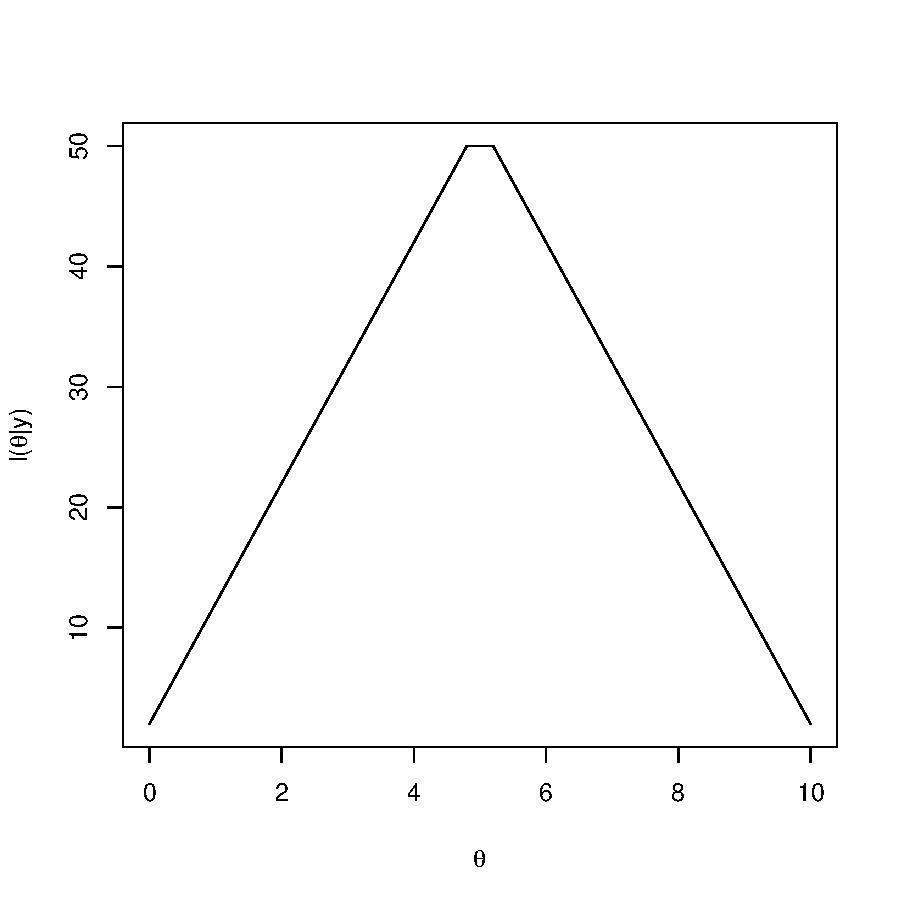
\includegraphics[width=2.5in, height=2.5in]{logit-ident.pdf}
\end{center}
\end{figure}
\pause
What's wrong with this?
\end{frame}

\begin{frame}
\frametitle{The Identification Problem}
\pause
There are more than one set of parameters that give the same maximum
likelihood value, so our model is \textbf{unidentified}. \\
\pause
\bigskip
Ordered Probit/Logit:
\pause
\begin{itemize}
\item If we estimate all the $\beta$s and $\tau$s, we can get many
sets of parameters that have the same likelihood. 
\pause
\item We can make our model identified in two ways:
\pause
\begin{itemize}
\item Fix $\beta_0 = 0$ and estimate all the $\tau$s (basically don't estimate an intercept) 
\pause
\item Fix $\tau_1 = 0$ and estimate an intercept.
\end{itemize}
\end{itemize}
\end{frame}

\end{document}
